\epigraph{\textit{The problem with interest rates is that you are not modeling a single number, you are modeling a whole term structure, so its a sort of different type of problem.}}{––\textsc{John Hull}, Professor of Risk Management \& Derivatives}

\section{Introduction}
In this chapter we explore interest rate derivatives––specifically swaps––in more detail, building on the mathematical foundations presented at the end of the previous chapter. We begin with a selective overview of some available products and the terminology used to describe them, before proceeding to discuss their pricing in more detail. We then consider the process of curve construction, describing two simple methodologies and produce a Python implementation based upon two historical datasets. Finally, we discuss some of the practical challenges faced and how our assumptions must be loosened before any real world application could be viable. 

\section{Terminology \& Products}
So far we have only spoken about interest rate derivatives in a general sense. Before considering the pricing of such derivatives, we must first understand the products available, their mechanics, and the associated terminology. The volume of products on offer is huge and as such we will not trouble ourselves by attempting to discuss and categorise them all, instead we will focus on those explored in this project. We summarise the detailed descriptions of the instruments presented in \cite{sadr2009interest}.

\subsection{Forward Rate Agreement}
A forward rate agreement is an OTC contract in which two parties agree a rate of interest to be paid for some specific time period, starting at some point in the future. The fixed rate of interest, which is agreed upon at the inception of the contract, is called the \textit{forward rate}. See definitions \ref{fwd_rate} and \ref{cont_fwd_rate}.

The future period for which the interest rate applies can be thought of as the borrowing and lending period. Forward rate agreements are quoted as $A \times B$, where $A$ represents the point from which the fixed forward rate applies, and $B$ represents the end of the contract.

\subsection{General Fixed-for-Floating Swap}
A general fixed-for-floating interest rate swap is an OTC agreement in which two parties agree to exchange a fixed rate of interest for a floating rate of interest. The floating rate of interest is tied to some benchmark reference rate and is set at the beginning of the interest period but paid at the end of the interest period. 

The cash flows on the either side of a fixed-for-floating interest rate swap are called \textit{legs}, and as such we will refer to the \textit{fixed leg} and the \textit{floating leg}. In addition, fixed-for-floating swaps are quoted from the perspective of the fixed leg. This means a swap for which an entity is paying the fixed rate has entered into a \textit{payer swap}. Likewise, a swap which receives the fixed rate is called a \textit{receiver swap}. 

At initiation, the fixed-for-floating swap is issued at par such that it has zero value to either party. The fixed rate of this swap, which we will refer to as the \textit{swap fixed rate}, is the price of the contract. 

The length of the contract is referred to as the \textit{term} or \textit{maturity} of a swap, while the frequency of the payments is called the \textit{tenor} of the swap. The fixed leg and the floating leg may have different tenors. The actual dollar amount of interest paid on each payment date is determined by the monies underlying the contract called the \textit{notional principle}. This notional principle is not exchanged at initiation of the contract. Furthermore, the two monetary interest payments are not typically exchanged, instead the two interest rates are netted and a single payment is made to the beneficiary.

\subsection{Overnight Indexed Swap}
An \textit{Overnight Indexed Swap} (`OIS') is a specific contract falling under the broader category of fixed-for-floating interest rate swaps described above. As the name suggests, the benchmark rate for an OIS is the overnight rate (of which there are multiple depending on the market) and the floating interest payments are a geometric average of the overnight rates during the interest period.

\subsection{Basis Swap}
Interest rate swaps need not necessarily have one fixed and one floating leg. A contract that has two floating legs, each tied to different benchmark rates, is called a \textit{basis swap}.

The two floating rates of a basis swap can be the \textit{same} benchmark rate but with \textit{different} tenors (e.g. 3M LIBOR vs.\ 6M LIBOR) or two \textit{different} benchmarks (e.g. 3M LIBOR vs.\ Commercial Paper). Often the two floating rates are denominated in the same currency, but benchmarks in two \textit{different} currencies are also possible (e.g. 3M-USD LIBOR vs.\ 3M-GBP LIBOR).

\subsection{General Interest Rate Swaption}
We can extend the concept of the swaps to consider swap options, or \textit{swaptions}. A swaption is the right, but not the obligation, to exercise the contract and enter into a fixed-for-floating interest rate swap. The terminology is analogous with that of the swap and a payer swaption is the right to enter the swap as the fixed rate payer, while a receiver swaption is the opposite. Clearly the optionality in the contract is valuable, hence, swaptions (as with options in general) require an upfront premium payment.

\subsection{Plain Vanilla vs. Exotic}
While each of the products above have different mechanics, they are all still considered standard by the market. That is, their features are simple, clearly understood, and used extensively by market participants. As such these contracts are classed as \textit{plain vanilla}. 

However, there may be times when a market participant has a very specific need and wishes to customise or tailor one of these contracts. By modifying the terms of the contract, it can no longer be classed as standardised, and is thus deemed to be \textit{exotic}.

Exotic features tend to reduce the liquidity of the contract and as such it may be difficult to close out the contract early should the need arise. Whether an exotic contract is cheaper or more expensive will depend on the nature of features added, that is, are they favourable for the purchaser. In addition, the exotic features make pricing such contracts far more challenging. 

\section{Pricing a Forward Rate Agreement}
The pricing of a forward rate agreement was innocuously covered in Chapter 2 when we discussed forward rates. This stems from the fact that the forward rate, calculated using discount factors and the concept of no arbitrage, is precisely the definition of a forward rate agreement. That is, the forward rate, $f(0,t_1,t_2)$, is an agreement to pay a fixed rate of interest starting at $t_1$ and ending at $t_2$. We repeat the prices here on a discretely compounded basis
\begin{equation}
    f_d(0, t_{i-1}, t_i) = \frac{\frac{Z(0, t_{i-1})}{Z(0,t_i)} - 1}{t_i - t_{i-1}}
\end{equation}
and on a continuously compounded basis
\begin{equation}
    f_{c}(0,t_{i-1}, t_i) = \frac{\ln [ Z(0,t_{i-1}) / Z(0,t_i)]}{t_i - t_{i-1}}.
\end{equation}

We will see in the next section that forward rate agreements can be used to price general fixed-for-floating interest rate swaps. 

\section{Pricing a General Fixed-for-Floating Swap}
Pricing an interest rate swap amounts to no more than the discounting of future cash flows. From our general introduction to a plain vanilla fixed-for-floating interest rate swap, we know that there are two streams of cash flows to consider: the (known) fixed interest payments and the (mostly unknown) floating interest payments.

Our aim is to find the appropriate fixed rate of interest that sets the present value of the fixed leg equal to the present value of the floating leg, thus giving the contract zero initial value. We consider each leg in turn.

\subsection{The Fixed Leg}
We will examine the fixed leg first, but before proceeding let us introduce some new notation to make our analysis less cumbersome. Following the convention of \cite{wilmott2013paul} we denote the swap fixed rate, $r_s$. In addition, we define the period of time between interest payments to be $\tau$. 

For our purposes we will consider payments which occur at the same time on both sides of the swap and thus simply writing $\tau$ will suffice. In practice, the fixed and floating legs will likely have different payment frequencies, hence, there will be two separate definitions of the time between interest payments. 

Recall the meaning of discount factors, $Z(0,t_i)$, from definition \ref{disc_fact}. To establish the present value of each of the fixed cash flows of the fixed leg we can use the corresponding discount factors. In doing so, we arrive at the following expression for the present value of the fixed leg.

\begin{definition}[Present value of the fixed leg]
\label{pv_fixed}
    Let $r_s$ be the annualised fixed rate of a plain vanilla fixed-for-floating interest rate swap. Let $\tau$ be the time period between interest payments. Then the present value of the fixed leg is given by,
    \begin{equation}
        PV_{\text{fixed}} = r_s \tau \sum_{i=1}^{N} Z(0,t_i). 
    \end{equation}
    Where $N$ represents the total number of interest payments during life of the contract. 
\end{definition}

\subsection{The Floating Leg}
The floating leg presents more of challenge since we are working with unknown future interest rates. From the description of the swap, we know that the floating rate of interest is set at the beginning of the interest period and paid at the end. However, as \cite{wilmott2013paul} points out, the underlying benchmark used to establish the floating rate payments is itself investable. This means we can appeal to the very definition of the benchmark rate. 

At the beginning of each interest period, we know the floating amount we will be required to pay. Now suppose we invest \$1 today at the prevailing floating rate. At the end of the interest period we will have \$1 plus the (time period scaled) return, which will exactly cover the floating interest payment. This means we can view each interest payment of the floating leg as a \$1 inflow at the start of the period and the outflow of \$1 at the end. 

This characterisation in terms of \$1 allows us to establish a link between floating leg payments and discount factors. An inflow at time $t_i$ has a present value of $+Z(0,t_i)$, while an outflow at time $t_{i+1}$ has a present value of $-Z(0,t_{i+1})$. As we repeat this over the life of the contract, it becomes a telescoping sum. This leads to the following definition. 

\begin{definition}[Present value of the floating leg]
\label{pv_float}
    Let $Z(0,t_i)$ be the discount factor associated with time $t_i$. Then the present value of a stream of floating interest rate payments is given by,
    \begin{align}
        PV_{\text{float}} &= \sum_{i=1}^{N} \left[ Z(0,t_{i-1})  - Z(0,t_{i})\right] \\
        &= Z(0, t_0) - Z(0, t_{N}) \\
        &= 1 - Z(0,t_N).
    \end{align}
\end{definition}

\subsection{The Price}
Returning to the question at hand, we are now in a position to determine the appropriate swap fixed rate, $r_s$. Equating the two present values
\begin{align}
    PV_{\text{fixed}} &= PV_{\text{float}} \\
    r_s \tau \sum_{i=1}^{N} Z(0,t_i) &= 1 - Z(0,t_N)
\end{align}
we arrive at the formula for a plain vanilla fixed-for-floating interest rate swap \citep{wilmott2013paul}
\begin{equation}
    r_s = \frac{1 - Z(0, t_N)}{\tau \sum_{i=1}^{N} Z(0,t_i)}.
\end{equation}

This representation of the swap fixed rate, $r_s$, using the discount factors (and associated discount curve) is not the only one. Using the relation between discount factors and forward rates, \cite{veronesi2016handbook} presents an equivalent formulation of the swap fixed rate,
\begin{equation}
    r_s = \frac{\sum_{i=1}^{N} Z(0,t_i) f(0,t_{i-1},t_i)}{\sum_{i=1}^{N} Z(0,t_i)}.
\end{equation}

To understand how these formulas are applied, the reader is referred to Appendix \ref{append_A3} which provides a detailed numerical example using both the discount factors and the forward rates. 

\subsection{A Note on Overnight Indexed Swaps}
Much of the pricing of Overnight Indexed Swaps is analogous to that of general fixed-for-floating swaps––an OIS is, after all, simply a specific instance of the general form. However, whilst general fixed-for-floating swaps may use LIBOR as a reference, meaning the rate for the interest period is known in advance, OIS use a sequence of daily overnight rates, hence, the future interest payment is not known until it is due. 

Using the notation of \cite{veronesi2016handbook}, we will denote $j = 1, \ldots, n$ to be the days in the interest period and $r_j$ to be the overnight rate associated with day $j$. Then the interest payment for an arbitrary time $t_i$ is given as,
\begin{equation}
    CF(t_i) = \prod_{j=1}^{n} \left( 1 + r_j \delta \right) - 1.
\end{equation}
Where $\delta$ is the time fraction corresponding to one day. 

The same argument still holds regarding the present values of the fixed and floating legs, only this time we rely on the discount curve associated with Overnight Indexed Swaps. We will refer to the OIS discount factors by the necessary superscript. We can compute the Overnight Indexed Swap fixed rate via
\begin{equation}
    r_{s}^{\text{OIS}} = \frac{1 - Z^{\text{OIS}}(0, t_N)}{\tau \sum_{i=1}^{N} Z^{\text{OIS}}(0,t_i)}
\end{equation}
using only OIS discount factors, and via
\begin{equation}
    r_{s}^{\text{OIS}} = \frac{\sum_{i=1}^{N} Z^{\text{OIS}}(0,t_i) f(0,t_{i-1},t_i)}{\sum_{i=1}^{N} Z^{\text{OIS}}(0,t_i)}
\end{equation}
using forward rates, just as before. 

\section{Pricing a Basis Swap}
The pricing of a Basis Swap follows a somewhat similar approach to a generic fixed-for-floating swap, only now we have two floating rates. As before, the swap is usually structured such that its value is zero at initiation, but what is its price? After all, there is no swap fixed rate to calculate. For basis swaps, the price is essentially the spread paid over one of the floating legs. 

When working with a basis swap of two different tenors of the same benchmark rate it may seem counter-intuitive to have any kind of spread, since there would appear to be an arbitrage opportunity. However, this spread reflects some of the subtler features of the market, namely the relative supply and demand of different tenors of the benchmark rate, in addition to some compensation for credit risk exposure.

The inclusion of a spread when the two benchmarks are different is a natural result given they will inherently have differing exposures and characteristics. In practice, with LIBOR-based basis swaps, the calculated spread, or price, is always added to the non-LIBOR side. 

\subsection{The LIBOR Floating Leg}
Once again, we are looking to determine present values. The pricing of the LIBOR floating leg follows exactly the same approach as that of the generic fixed-for-floating swap in definition \ref{pv_float}.

\subsection{The Alternative Floating Leg}
Let us introduce some further notation. We define the alternative reference rate, $r^{alt}(t_i)$ and the spread, $m$, following the convention of \cite{flavell2012swaps}. Similarly to the fixed leg of a generic fixed-for-floating swap, we are discounting a series of cash flows. Unfortunately, this time they are a sequence of variable unknown future cash flows, so we cannot move $r^{\text{alt}}(t_i)$ outside of the sum. Instead we can simply write
\begin{equation}
    PV_{\text{alt}} = \tau \sum_{i=1}^{N} \left( r^{\text{alt}}(t_i) + m \right) Z(0,t_i).
\end{equation}
Where $\tau$ represents the time between interest payments, as before.

\subsection{The Price}
Equating the two floating rates, we arrive at the following equation
\begin{align}
    PV_{\text{float}} &= PV_{\text{alt}} \\
    1 - Z(0,t_N) &= \tau \sum_{i=1}^{N} \left( r^{\text{alt}}(t_i) + m \right) Z(0,t_i).
\end{align}
It turns out that we cannot simply invert this equation to find the appropriate spread, $m$, and must use optimisation and numerical methods to do so. In practice, these spreads are already quoted in the market and thus our main task is inferring the appropriate forward curve for the alternative benchmark––using a technique called \textit{bootstrapping} (discussed shortly).

\section{Curve Construction}
With the formulas presented above you could be forgiven for thinking that the pricing of those interest rate derivative contracts is straightforward. Given a starting point, say, a set of discount factors, one could compute fair prices using little more than a spreadsheet. 

The real challenge lies in establishing the correct starting point. Recall, throughout our discussions of forward rates, spot rates, and discount factors we have not mentioned where they come from in the first place. Can they simply be observed in the market? Sadly, the answer is no. 

It turns out that our presentation so far needs to be reversed. Instead of using the discount factors or other rates to find the prices of products like fixed-for-floating swaps, we must use the prices of those swaps to find the discount factors and rates. 

We can take this approach in large part due to the size and liquidity of the interest rate derivatives market discussed in Chapter 2. The market is sufficiently large that products such as swaps are, in fact, priced by the principles of supply and demand, independent of any models \citep{wilmott2013paul}. As such, we use the market quoted rates on various interest rate instruments to compute discount factors and rates, and \textit{construct their associated curves}. This then allows us to price back any contracts, not just those observable in the market. 

\subsection{Methodology}
Constructing \textit{appropriate} curves is a challenging feat, partly due the limited number of available instruments in comparison to the number of points required to properly cover the length of the curve. We will discuss the specifics shortly, but in general the method proceeds as follows \citep{banque_canada}. For the purposes of our project, we will use a continuously compounded basis.

\subsubsection{Choosing Appropriate Instruments}
The first step is to decide on a set of interest rate instruments to be used as inputs. We have mentioned the liquidity of interest rate derivatives in general, but of course some will be more liquid than others. The concept of stale pricing––that is, financial instruments which do not trade actively and therefore their quoted price may not be representative of current market conditions––is of serious concern, since they are likely to produce incorrect curves. 

To identify the best products, the curve can be split into three sections, comprising of the short, medium, and long term. For the short term, deposit instruments such as LIBOR rates could be used as these were previously available up to one year. For the medium term, either forward rate agreements or Eurodollar futures (adjusted for convexity) could be used, constituting somewhere between six months and two years––if overlapping instruments are used, the result is a \textit{blended curve}. In the long term, from one or two years and beyond, swap rates are used. 

\subsubsection{Constructing the Short Section}
At the short end of the curve, we are fortunate that the instruments chosen, say LIBOR deposit rates, are inherently zero coupon. This means we can extract both the spot rates and the discount factors directly using the results from Chapter 2.

Let $\ell(t_i)$ be the LIBOR rate associated with time $t_i$. Then we can compute the spot rate via
\begin{equation}
    r_c(t_i) = \frac{1}{t_i} \ln ( 1 + \ell(t_i) t_i).
\end{equation}
Which can then be used to compute the discount factor through
\begin{equation}
    Z(0,t_i) = e^{-r_c(t_i) t_i}.
\end{equation}
Alternatively, we can jump directly from the LIBOR rate to the discount factor using
\begin{equation}
    Z(0,t_i) = \frac{1}{1 + \ell(t_i) t_i}.
\end{equation}

\subsubsection{Constructing the Middle Section}
We have a choice of approaches for the middle section of the curve. If we use forward rate agreements then we can extend our discussion of forward rates in Chapter 2 and invert definition \ref{cont_fwd_rate} to express discount factors in terms of forward rates
\begin{equation}
    Z(0,t_i) = Z(0,t_{i-1}) e^{- f_c(0,t_{i-1},t_i) (t_{i-1} - t_i)}.
\end{equation}
We can proceed recursively, noting that $Z(0,0) = 1$ to find that
\begin{align}
    Z(0,t_i) &= \prod_{j=1}^{i-1} e^{- f_c(0,t_{i-1},t_i) (t_{i-1} - t_i)} \\
    &= \exp \left( - \sum_{j=1}^{i-1} f_c(0,t_{i-1},t_i) (t_{i-1} - t_i) \right).
\end{align}
Hence, we can find the discount factors and obtain spot rates and forward rates through the usual means.

Since forward rate agreements are OTC instruments, they are not subject to the conditions of exchanges. An alternative to forward rate agreements is to use Eurodollar futures contracts. By definition, futures contracts are exchange traded and thus are marked-to-market at the end of each day, with gains and losses being reflected in the margin account of each counterparty. This daily fluctuation bring about additional opportunities as gains can be reinvested at higher rates of return, on the other hand losses can be financed at lower rates \citep{piterbarg2004eurodollar}. The asymmetrical nature of this technical feature means that Eurodollar futures values contain convexity––that is, the value will rise by a greater amount than it would fall given equal and opposite movements––a second order effect. 

In practice, this requires an adjustment to the value of the Eurodollar futures contracts. The specific adjustment applied depends on the choice of short term interest rate model, however, generally speaking the change is minimal for shorter maturities (in the region of a few basis points) and so its true implications are beyond the scope of this project. The interested reader is referred to \cite{hull2003options} and \cite{piterbarg2004eurodollar} for a more detailed treatment.

We must convert the quoted rate to a continuous basis, noting they settle quarterly on specific fixed days of the month, and then apply the following recursive formula to generate the spot rate. We will denote $EF(t_i)$ be the continuous Eurodollar future rate,
\begin{equation}
    r_c(t_i) = \frac{EF(t_i) (t_i - t_{i-1}) + r_c(t_{i-1}) t_{i-1}}{t_i}.
\end{equation}
Once again, we can obtain the discount factors and forward rates from their respective formulas. 

\subsubsection{Constructing the Long Section}
To construct the long end of the curve we turn to fixed-for-floating swap quotes. Returning to our swap pricing formula and inverting, we obtain
\begin{equation}
    Z(0,t_i) = \frac{1 - r_s(t_i) \tau \sum_{j=1}^{i-1} Z(0,t_j)}{1 + r_s(t_i) \tau}.
\end{equation}
In words, this means we can iteratively compute the discount factor associated with time $t_i$ using the market quoted swap rate, $r_s(t_i)$, the time between interest payments $\tau$, and the discount factors associated with all interest payments prior to that time. This progressive method, which uses all previously obtained discount factors to compute the next one, is called \textit{bootstrapping} \citep{wilmott2013paul} \citep{veronesi2016handbook}.

\subsubsection{Interpolation Schemes}
At first glance this curve construction technique seems intuitive. We simply begin by computing the discount factors and spot rates at the short end and proceed along the curve utilising what we have previously calculated. 

Unfortunately, any implementation of such method will soon run into a problem. At the longer end of the curve, we require the discount factors associated with \textit{every interest payment over the life of the swap} (excluding the final payment of course, which is what we are trying to work out). But it is highly unlikely that there are liquid quotes for all of these times.

Consider a 15-year swap with semi-annual fixed and floating interest payments. Suppose we find that the most liquid swap maturity prior to this is 12-years. We may have computed the discount factors for every six month period from initiation to 12-years, but cannot continue further due to the lack of data. We still need the discount factors for 12.5, 13, 13.5, 14, and 14.5, hence, we must \textit{interpolate} between these points. 

Which interpolation technique to use is not a decision to be taken lightly. This presents the biggest challenge during curve construction of which there is no universally agreed correct answer. \cite{hagan2006interpolation} conducted extensive analysis into the different interpolation methods used in curve construction, ranging from simple linear interpolation to more complicated monotone convex interpolation––which is used by the U.S. Department of the Treasury for their yield curve construction \citep{us_treas}. The interested reader can find a concise comparison of the many different methods in \cite{hagan2008methods}. As our project is focused on the pricing of interest rate swaps, rather than analysing and evaluating different curve construction techniques, there is insufficient benefit in considering the complex, optimisation based approaches and instead we will focus on two simple, but still popular, methods: linear interpolation and cubic spline interpolation \citep{flavell2012swaps}. 

Given the interlinked nature of discount factors and spot rates we must also decide \textit{which} to interpolate. We can interpolate the discount factors directly, or we can interpolate the spot rates and infer the appropriate discount factors from those. 

\subsection{Python Implementation}
Having covered the general curve construction methodology, we can now move on and consider its computational implementation in more detail. We have used Python and describe our step-by-step curve construction in words, before presenting the pseudocode. We then discuss the results of a real-world example. Our full code can be found in Appendix \ref{python_code}.

\subsection{Step-by-Step Curve Construction}
\textbf{Method:} Interpolation of the discount factors, or \textit{explicit discount factor} method.
\begin{enumerate}
    \item \textbf{Short Section:} Compute the discount factors and spot rates for the short section of the curve using the using the approach outlined in Section 3.6.1.2. 
    \item \textbf{Middle Section:} Compute the discount factors and spot rates for the middle section of the curve using either of the two approaches outlined in Section 3.6.1.3 depending on the intermediate instruments being used.
    \item \textbf{Long Section:}
    \begin{enumerate}
        \item Identify the term of the swap being used for the long section of the curve, $t_i$.
        \item Identify the frequency of the interest payments of the swap, say $n$.
        \item Construct an array containing the interest payment times up to, but not including, the final interest payment, say, $\textbf{p} = \left[ \frac{1}{n}, \frac{2}{n}, \ldots, \frac{n t_i - 1}{n} \right]$. We will define $p_j, \text{ where } j = 1, \ldots i-1$, as the j\textsuperscript{th} interest payment.
        \item Construct an array of all the times associated with the discount factors computed so far, say $x$.
        \item Construct an array of all the discount factors at those times, say $y$.
        \item Interpolate $(x,y)$ using the intended method (e.g. linear or cubic spline). We used the SciPy package available in Python. 
        \item Initialise a dummy variable to store the sum of the discount factors, $DF = 0$.
        \item Perform a \textit{for} loop over the interest payment times, $p_j$, evaluating the discount factor, $Z(0,p_j)$, on the interpolated curve of $(x,y)$, and summing the result, $DF = \sum_{j=1}^{i-1} Z(0,p_j)$.
        \item Compute the final bootstrapped discount factor associated with $t_i$ using the formula in Section 3.6.1.4
        \item Repeat from step 3(a) for the next swap maturity.
    \end{enumerate}
\end{enumerate}

We can present the construction of the long end in a more concise manner using pseudocode.

\begin{algorithm}
\caption{Constructing the Long Section: Explicit Discount Factors}\label{alg:boot_dfs}
    \begin{algorithmic}[1]
    \Require $t_i$
    \Require $n$ \Comment{Frequency of interest payments}
    \Require $r_s(t_i)$

    \State $\textbf{p} = [\frac{1}{n}, \frac{2}{n}, \ldots, \frac{n t_i - 1}{n}]$ \Comment{Interest payment dates}
    \State $\tau = p_j - p_{j-1} $ \Comment{Assume constant for our purposes}
    \State $x \gets$ `times'
    \State $y \gets$ `discount factors'
    \State Interpolate $(x,y)$

    \State $DF = 0$
    \For{$j = 1, \ldots, i-1$} 
        \State Extract $Z(0,p_j)$ from curve
        \State $DF = DF + Z(0,p_j)$ 
    \EndFor

    \State $Z(0,t_i) = \frac{1 - r_s(t_i) \tau DF}{1 + r_s(t_i) \tau}$
    \Repeat
    \Until{Curve construction complete.}
    \end{algorithmic}
\end{algorithm}

\FloatBarrier

Alternatively, we can interpolate the spot rates. The construction of the short and middle sections remain the same, so we must only alter the method for the long section. \\[8pt]
\textbf{Method:} Interpolation of the spot rates and inference of the discount factors, or \textit{implicit discount factor} method.

\begin{enumerate}
    \setcounter{enumi}{2}
    \item \textbf{Long Section:}
    \begin{enumerate}
        \item Identify the term of the swap being used for the long section of the curve, $t_i$.
        \item Identify the frequency of the interest payments of the swap, say $n$.
        \item Construct an array containing the interest payment times up to, but not including, the final interest payment, say $\textbf{p} = \left[ \frac{1}{n}, \frac{2}{n}, \ldots, \frac{n t_i - 1}{n} \right]$. We will define $p_j, \text{ where } j = 1, \ldots i-1$, as the j\textsuperscript{th} interest payment.
        \item Construct an array of all the times associated with the \textit{spot rates} computed so far, say $x$.
        \item Construct an array of all the \textit{spot rates} at those times, say $y$.
        \item Interpolate $(x,y)$ using the intended method (e.g. linear or cubic spline). We used the SciPy package available in Python. 
        \item Initialise a dummy variable to store the sum of the discount factors, $DF = 0$.
        \item Perform a \textit{for} loop over the interest payment times, $p_j$, evaluating the \textit{spot rate}, $r_c(p_j)$ on the interpolated curve of $(x,y)$. \textit{Convert that spot rate into a discount factor}, $Z(0,p_j)$, and sum the result, $DF = \sum_{j=1}^{i-1} Z(0,p_j)$.
        \item Compute the final bootstrapped discount factor associated with $t_i$ using the formula in Section 3.6.1.4
        \item Repeat from step 3(a) for the next swap maturity.
    \end{enumerate}
\end{enumerate}

Once again, this step can be concisely presented as pseudocode.

\begin{algorithm}
\caption{Constructing the Long Section: Implicit Discount Factors}\label{alg:boot_zsr}
    \begin{algorithmic}[1]
    \Require $t_i$
    \Require $n$ \Comment{Frequency of interest payments}
    \Require $r_s(t_i)$

    \State $\textbf{p} = [\frac{1}{n}, \frac{2}{n}, \ldots, \frac{n t_i - 1}{n}]$ \Comment{Interest payment dates}
    \State $\tau = p_j - p_{j-1} $ \Comment{Assume constant for our purposes}
    \State $x \gets$ `times'
    \State $y \gets$ `spot rates'
    \State Interpolate $(x,y)$

    \State $DF = 0$
    \For{$j = 1, \ldots, i-1$} 
        \State Extract $r_c(p_j)$ from curve
        \State Convert $r_c(p_j) \longrightarrow Z(0,p_j)$
        \State $DF = DF + Z(0,p_j)$ 
    \EndFor

    \State $Z(0,t_i) = \frac{1 - r_s(t_i) \tau DF}{1 + r_s(t_i) \tau}$
    \Repeat
    \Until{Curve construction complete.}
    \end{algorithmic}
\end{algorithm}

\subsection{Datasets}
For our implementation, we have used two datasets as this will allow us to compare the differences in curve construction under two separate scenarios.

The first dataset is a combination of USD LIBOR rates, obtained from \cite{usd_libor}, and mid-quotes on USD fixed-for-floating LIBOR-based swaps obtained from \cite{flavell2012swaps}, with the underlying data from ICAP, on the 15\textsuperscript{th} February 2008. Note for this first dataset, our curve will be only be constructed from deposit rates and swaps. That is, we will omit any FRA or Eurodollar future quotes and simply interpolate between the short and long sections.

Our second dataset is a combination of USD LIBOR rates, a selection of Eurodollar futures quoted rates, and mid-quotes on USD fixed-for-floating LIBOR-based swaps, once again obtained from \cite{flavell2012swaps}, on the 6\textsuperscript{th} February 2008. This time our curve will be constructed using short, medium, and long instruments. Tables containing both sets of data can be found in Appendix \ref{datasets}.

\subsection{Results}

Figures \ref{fig:curves_1}, \ref{fig:curves_2}, \ref{fig:curves_3}, and \ref{fig:curves_4} show the results of our curve constructions for the two datasets. Tables containing detailed numerical results can be found in Appendix \ref{results}. 
%It is worth noting that we can be confident in the output as their shape appears to be a close match to that given in \cite{flavell2012swaps}––they will not be identical as we have chosen simplified assumptions for both the frequency and time between interest payments.

From Figure \ref{fig:curves_1} we can see from both panels that the spot curves under all four construction techniques appear smooth with only marginal differences between the rates across all maturities. However, the same is not true for the forward curve in Figure \ref{fig:curves_3}.

We need only consider the forward curve out to 10-years to get a clear understanding of the impacts of the different construction techniques. We notice that the Explicit Discount Factor method (both linear and cubic spline) and the linear Implicit Discount Factors produce a smooth, appropriate-looking forward curve, however, we begin to see instability under the cubic spline Implicit Discount Factor method. 

This wave-like curve structure stems from the fact that, at the short end, the discount factors used to compute forward rates are close together, hence,  minor differences can dominant and noticeably alter the forward rate. As the time extends, the differential between discount factors plays a less important role and we can see convergence under all four techniques. 

Turning our attention to Figure \ref{fig:curves_2}, both panels indicate the long end of spot curve is once again smooth, however, this time the shorter end is not. This follows from the choice of instruments used, as dataset 1 only contained LIBOR deposit rates and swaps, whereas dataset 2 included Eurodollar futures in the time period between 1- and 2-years. Whilst this provides additional information, since these are market quoted prices, it highlights the challenges faced when stitching the different sections of the curve together. In practice, the instruments may be chosen such that they overlap, creating a blended curve, to compensate for the different contracts.

This issue pales in comparison to the jagged nature of the forward rate curve. As we can see from Figure \ref{fig:curves_4}, all four construction methodologies give unstable and inappropriate forward curves. This highlights the sensitive nature of the forward curves as there is apparently little difference between the data used to produce this forward curve on 06/02/2008 and less than ten days later on 15/02/2008, yet the latter appears relatively smooth, while the former is particularly unstable.

The inappropriate appearance of this curve does not invalidate the fact that both curves produced can be considered no-arbitrage forward curves for the instruments used in their construction. That is, using the forward curve and its associated discount curve under any of the methodologies, we can price back those same instruments to the observed market rates.

Clearly, however, it will not produce a reasonable price for those instruments \textit{not} used in its construction. And therein lies the challenge. We are faced with a trade-off between strictly following the steps to construct the curve, and facing whatever forward curve stems as a result, or try and control the appearance of the curve and bear the consequences that it will no longer be considered free of arbitrage opportunities. In practice, this is a fine balance, and one in which the use of optimisation plays a major role. 

\begin{figure}[ht]
\begin{center}
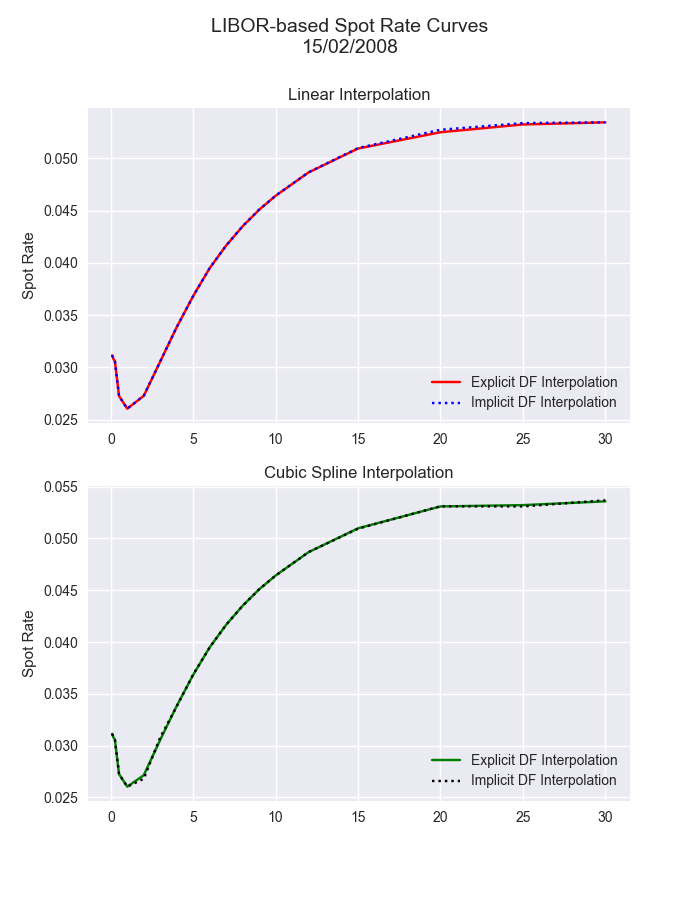
\includegraphics[width=0.8\textwidth, trim={1.8cm 2cm 1.8cm 2.5cm}]{Chapter_3/images/spot_graph1.png}
\caption[LIBOR-based Spot Rate Curves using different construction techniques on 15/02/2008]{LIBOR-based Spot Rate Curves on 15/02/2008. \textbf{Panel 1}––The spot rate curves constructed using linear interpolation of the discount factors (`Explicit DF') and linear interpolation of the spot rates and inference of discount factors (`Implicit DF'). \textbf{Panel 2}––The spot rate curves constructed using cubic spline interpolation of the discount factors (`Explicit DF') and cubic spline interpolation of the spot rates and inference of discount factors (`Implicit DF').}
\label{fig:curves_1}
\end{center}
\end{figure}

\begin{figure}[ht]
\begin{center}
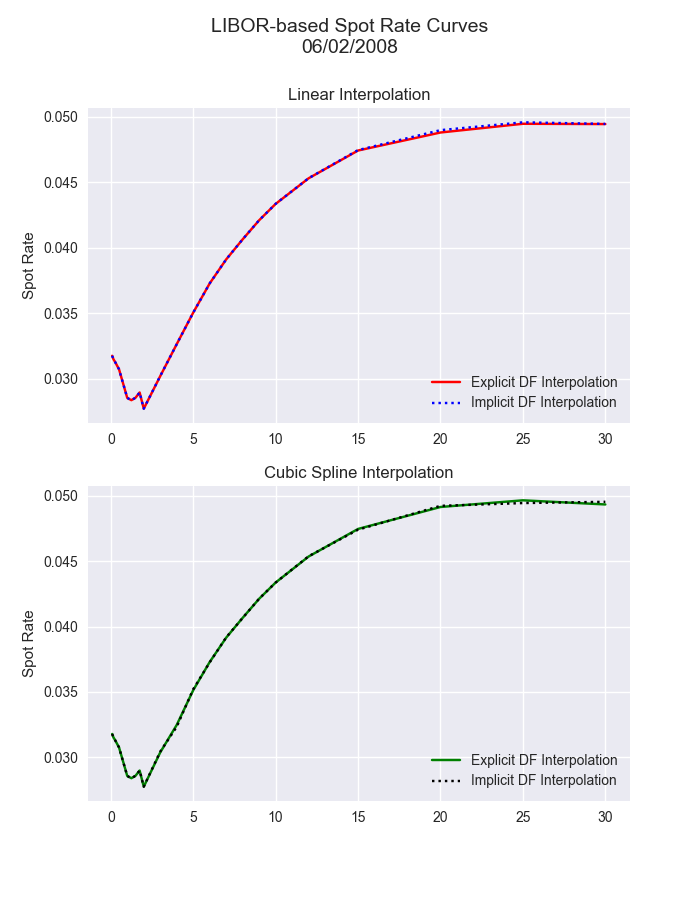
\includegraphics[width=0.8\textwidth, trim={1.8cm 2cm 1.8cm 2.5cm}]{Chapter_3/images/spot_graph2.png}
\caption[LIBOR-based Spot Rate Curves using different construction techniques on 06/02/2008]{LIBOR-based Spot Rate Curves on 06/02/2008. \textbf{Panel 1}––The spot rate curves constructed using linear interpolation of the discount factors (`Explicit DF') and linear interpolation of the spot rates and inference of discount factors (`Implicit DF'). \textbf{Panel 2}––The spot rate curves constructed using cubic spline interpolation of the discount factors (`Explicit DF') and cubic spline interpolation of the spot rates and inference of discount factors (`Implicit DF').}
\label{fig:curves_2}
\end{center}
\end{figure}

\begin{figure}[ht]
\begin{center}
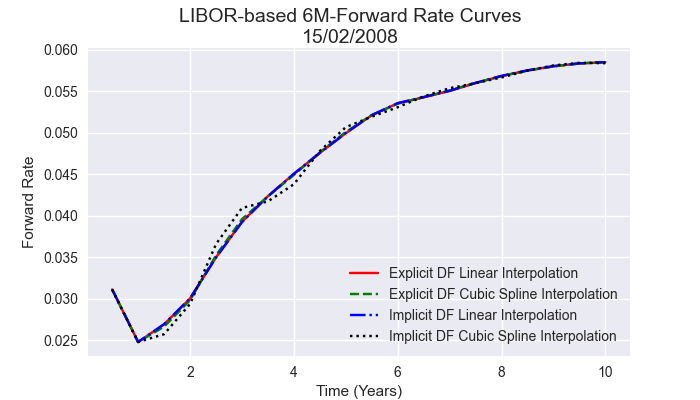
\includegraphics[width=0.8\textwidth, trim={1.8cm 0cm 1.8cm 2.5cm}]{Chapter_3/images/fwd_graph1.png}
\caption[LIBOR-based 6M-Forward Curves using different construction techniques on 15/02/2008]{LIBOR-based 6M-Forward Rate Curves on 15/02/2008 associated with each of the four construction techniques.}
\label{fig:curves_3}
\end{center}
\end{figure}

\begin{figure}[ht]
\begin{center}
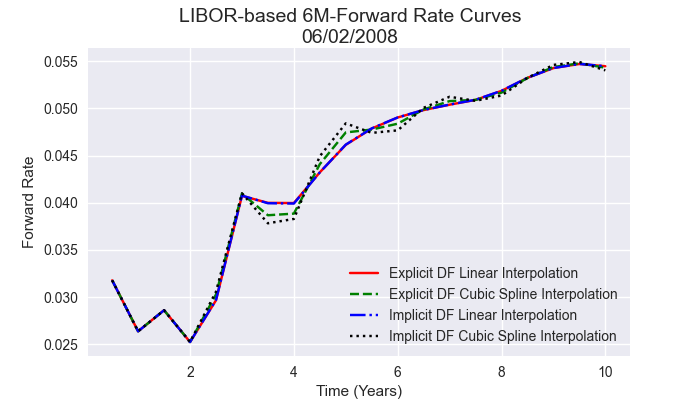
\includegraphics[width=0.8\textwidth, trim={1.8cm 0cm 1.8cm 2.5cm}]{Chapter_3/images/fwd_graph2.png}
\caption[LIBOR-based 6M-Forward Curves using different construction techniques on 06/02/2008]{LIBOR-based 6M-Forward Rate Curves on 06/02/2008 associated with each of the four construction techniques.}
\label{fig:curves_4}
\end{center}
\end{figure}

\FloatBarrier

\section{Practical Considerations}
Our Python implementation is a useful tool for illustrating the curves constructed from the different methodologies. However, our underlying assumptions mean it is a simplified version of the problem faced in the real-world. In this section we discuss some of the additional factors that must be considered and describe how those changes could be incorporated.

\subsection{Day Count Convention}
A major component of curve construction is the instruments used. If we dig a little deeper into those products, and consider their settlement characteristics in more detail, we find several complications relating to day count convention.

For our purposes we assumed that a year consisted of 360 days and each month was 30 days. This allowed us to consider months as simple fraction, for instance 3-months is simply 0.25. In practice, however, this may not always be the case. Different products use different conventions––actual/360 and actual/365 are just a couple of the possibilities, where actual refers to the actual number of days between two dates. 

In addition, we must consider the concept of business days, and factor in things such as public holidays for the market in question. As a result, not only do we need to know the quoted swap rates to be used in our curve construction, we must also gather the relevant payment and settlement information and compute the true length of time where required. Whilst this adjustment is not conceptually difficult, its implementation requires a great deal of care.

\subsection{Asymmetrical Interest Payments}
When constructing the long section of the curve we made the simplifying assumption that interest payments on both the fixed and floating sides of the swaps were made semi-annually. This does not have to be (and usually is not) the case. 

For instance, the fixed leg of a generic USD swap is paid semi-annually, whereas the floating rate leg is paid quarterly. This complicates our curve construction somewhat, as our initial interpolation between swap rates would be on an \textit{semi-annual} basis, but we may be interested in the quarterly forward curve associated with the LIBOR fixing of the floating rate side. We would then need to make a further decision about the interpolation between the calculated discount factors. 

\newpage

As we saw in Figures \ref{fig:curves_3} and \ref{fig:curves_4}, the forward curve is particularly sensitive and this interest payment complexity can cause the forward curve to become erratic. In fact, it is the stabilisation and appropriate construction of the forward curve that demands the most attention and, in general, a combination of interpolation techniques and optimisation methods may be used. 

To summarise the challenges faced by day count conventions and interest payment frequencies, we display the following table based on the information given in \cite{sadr2009interest}.

\vspace{1cm}

\begin{table}[ht]
\begin{center}
\begin{tabular}{ccccc}

\toprule
 & \textsc{Fixed Leg} & \textsc{Float Leg} & & \\
\multirow{2}{*}{\textsc{Currency}} & \textsc{Freq \&} & \textsc{Freq \&} & \textsc{Float Leg} & \multirow{2}{*}{\textsc{Spot Date}} \\
 & \textsc{Day Count} & \textsc{Day Count} & \textsc{Index} & \\
\toprule

\multirow{2}{*}{USD} & S/A & Q & \multirow{2}{*}{USD 3m LIBOR} & \multirow{2}{*}{2d LONDON} \\
& 30/360 & Act/360 & & \\

\multirow{2}{*}{EUR} & A & S/A & \multirow{2}{*}{EUR 6m LIBOR} & \multirow{2}{*}{2d Target} \\
& 30/360 & Act/360 & & \\

\multirow{2}{*}{EUR-1Y} & \multirow{2}{*}{Single} & Q & \multirow{2}{*}{EUR 3m LIBOR} & \multirow{2}{*}{2d Target} \\
& & Act/360 & & \\

\multirow{2}{*}{JPY} & S/A & S/A & \multirow{2}{*}{JPY 6m LIBOR} & \multirow{2}{*}{2d TOK} \\
& Act/365 & Act/360 & & \\

\multirow{2}{*}{GBP} & S/A & S/A & \multirow{2}{*}{GBP 6m LIBOR} & \multirow{2}{*}{Same Day} \\
& Act/365 & Act/365 & & \\

\multirow{2}{*}{GBP-1Y} & Q & Q & \multirow{2}{*}{GBP 3m LIBOR} & \multirow{2}{*}{Same Day} \\
& Act/365 & Act/365 & & \\

\multirow{2}{*}{CHF} & A & S/A & \multirow{2}{*}{CHF 3m LIBOR} & \multirow{2}{*}{2d ZUR} \\
& 30/360 & Act/360 & & \\

\toprule

\end{tabular}
\end{center}
\caption[Summary: Day Count Conventions and Interest Payment Frequencies]{A summary of the different day count conventions and payment frequencies of general fixed-for-floating interest rate swaps in major markets.}
\label{tab:dcc_irp}
\end{table}

\vspace{0.5cm}

\subsection{Single vs. Multi-curve Pricing}
The approach that we have been discussing so far is the so called \textit{single curve framework}. That is, we are using observable market quotes for LIBOR based instruments and constructing the curve which then prices those same instruments under the assumption of no arbitrage. This approach was popular prior to the financial crisis when LIBOR rates were assumed to be representative of risk-free rates.

After the financial crisis, however, LIBOR rates were no longer deemed truly risk-free and as such the market moved towards the \textit{multi-curve framework}. This involved using observed OIS quotes to construct the discount curve, computing the associated forward rates from a combination of the OIS discount curve and observed LIBOR-based swap quotes, before inferring the LIBOR-based discount factors and spot curve.

We can distinguish the two frameworks by their respective flow charts, summarised from \cite{veronesi2016handbook}.

\begin{figure}[ht]
\begin{center}
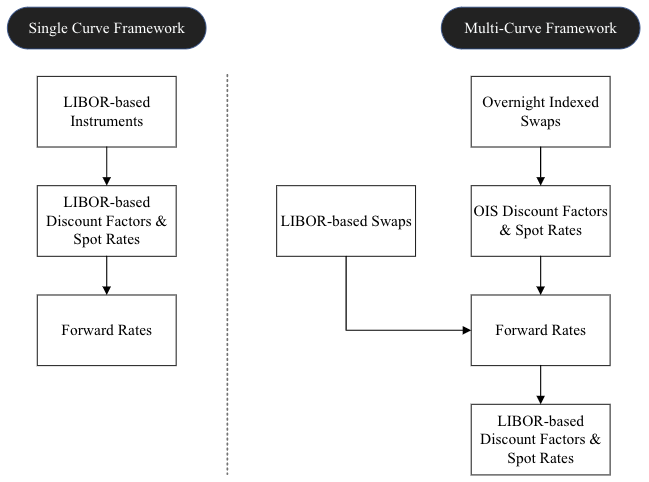
\includegraphics[width=0.9\textwidth]{Chapter_3/images/Pre_Post FC.png}
\caption[Comparison of single and multi-curve frameworks]{A flowchart depicting the difference between the single curve and multi-curve frameworks. The single curve was used extensively prior to the financial crisis, however, the multi-curve approach has been used since owing to LIBOR rates not being deemed truly risk-free.}
\label{fig:pre_post}
\end{center}
\end{figure}
